\chapter{Foundations of Linear Algebra for Machine Learning:\
A Constructivist and Intuitionist Approach (Andrew Ng notation)}

\begin{quote}
    \emph{``Mathematical objects are not discovered in a Platonic realm; they are constructed through systematic mental activity, emerging from our intellectual need to represent and transform structure.''}\\
    \hfill--- L.E.J. Brouwer, \textit{Intuitionism and Formalism} (1912)
\end{quote}

\vspace{1em}

\noindent\textbf{Chapter Overview:} This chapter develops linear algebra from foundational principles to advanced decompositions, integrating the constructivist--intuitionist philosophy with Andrew Ng's machine learning notation. We emphasize that mathematical objects—vectors, matrices, transformations—are \textit{constructed entities} designed to encapsulate structure and enable computation. Our notation distinguishes structural position (subscripts) from semantic identity (superscripts), mirroring the separation between architecture and instances in deep learning.

\section{Philosophical Prolegomenon: Constructivism and Mathematical Objects}

\subsection{The Constructivist Imperative}

\begin{philobox}
    \textbf{Constructivism in Mathematics and Machine Learning}

    The constructivist program, initiated by Kronecker and formalized by Brouwer,
    asserts:

    \begin{enumerate}
        \item \textbf{Existence requires construction:} A mathematical object exists if and only if we can construct it through explicit, finite procedures.

        \item \textbf{Truth requires proof:} A proposition is true if and only if we can construct a proof. The Law of Excluded Middle ($P \vee \neg P$) is rejected unless we can decide $P$ constructively.

        \item \textbf{Mental constructions precede notation:} Symbols represent mental constructions; they do not have independent existence.
    \end{enumerate}

    \textbf{Relevance to Machine Learning:}

    In machine learning, constructivism manifests naturally:
    \begin{itemize}
        \item A neural network with parameters $\theta$ exists because we \textit{construct}
              it: we initialize $\theta^{[0]}$, then iteratively construct $\theta^{[1]},
                  \theta^{[2]}, \ldots$ via gradient descent.
        \item A representation $\vect{x}^{(i)} \in \mathbb{R}^n$ for a data point is a
              \textit{constructed encoding}, not a discovered truth.
        \item Training is iterative construction: from data $\{(\vect{x}^{(i)},
                  y^{(i)})\}_{i=1}^m$, we construct a function $f_\theta: \mathbb{R}^n \to
                  \mathbb{R}^k$.
    \end{itemize}

    This philosophical stance guides our pedagogy: we build each concept
    explicitly, showing how it arises from intellectual necessity.
\end{philobox}

\subsection{Intuitionism and the Nature of Mathematical Truth}

\begin{intuitionbox}
    \textbf{Brouwer's Intuitionism}

    For Brouwer, mathematics is a ``languageless activity of the mind.'' Key
    tenets:
    
    \begin{itemize}
        \item \textbf{Rejection of actual infinity:} Infinite sets are not completed objects but potential processes. The set $\mathbb{N}$ represents an \textit{ongoing construction}, not a finished totality.

        \item \textbf{Logical vs. mathematical truth:} Classical logic (with excluded middle) applies to finite constructions. For infinite domains, we need intuitionistic logic.
    \end{itemize}

    \textbf{Implication for Linear Algebra:}

    A vector space $V$ of dimension $n < \infty$ is fully constructible: we can
    explicitly list a basis $\{\vect{b}_1, \ldots, \vect{b}_n\}$ and construct
    every $\vect{v} \in V$ as:
    \[
        \vect{v} = \sum_{j=1}^{n} c_j \vect{b}_j, \quad c_j \in \mathbb{R}
    \]

    This construction is finite, explicit, and algorithmic—perfectly aligned with
    computational practice in machine learning.
\end{intuitionbox}

\section{The Transition from Numbers to Abstract Objects}

\subsection{The Nature of Mathematical Objects: From Scalars to Vectors}

\subsubsection{Scalars: The Foundation}

\begin{definition}[Scalar]
    A \textbf{scalar} is an element of a field $\mathbb{F}$, typically $\mathbb{R}$ (real numbers) or $\mathbb{C}$ (complex numbers). In machine learning contexts, $\mathbb{F} = \mathbb{R}$ unless otherwise specified.

    \textbf{Notation:} Scalars are denoted by lowercase Latin or Greek letters: $a, b, c, \alpha, \beta, \theta$.

    \textbf{Construction:} Real numbers are constructed via Dedekind cuts or Cauchy sequences—explicit, finitary procedures defining infinite decimals.
\end{definition}

\begin{intuitionbox}
    \textbf{Why Scalars Are Insufficient for Machine Learning}

    Consider predicting house prices. A single feature (e.g., area in m²) gives:
    \[
        \text{price} = \theta_0 + \theta_1 \cdot \text{area}
    \]

    But real prediction requires multiple features:
    \begin{itemize}
        \item Area: $x_1^{(i)}$ m²
        \item Number of bedrooms: $x_2^{(i)}$
        \item Distance to city center: $x_3^{(i)}$ km
        \item Age of building: $x_4^{(i)}$ years
    \end{itemize}

    We need a structure to encapsulate $(x_1^{(i)}, x_2^{(i)}, x_3^{(i)},
        x_4^{(i)})$ as a single object. This intellectual necessity drives the
    construction of vectors.
\end{intuitionbox}

\subsubsection{Vectors: Encapsulating Multi-Symbol Objects}

\begin{notationbox}
    \textbf{Andrew Ng Notation Convention for Vectors}

    \begin{itemize}
        \item \textbf{Superscripts} denote \textit{semantic identity} (which example, which class, which layer):
              \[
                  \vect{x}^{(i)} = \text{the } i\text{-th training example}
              \]

        \item \textbf{Subscripts} denote \textit{structural position} (which component, which row/column):
              \[
                  x_j^{(i)} = \text{the } j\text{-th feature of example } i
              \]

        \item \textbf{Bold lowercase} indicates vectors:
              \[
                  \vect{x}, \vect{y}, \vect{a}, \vect{b}, \vect{w}, \vect{v}
              \]

        \item \textbf{Column vector default:}
              \[
                  \vect{x}^{(i)} = \begin{bmatrix} x_1^{(i)} \\ x_2^{(i)} \\ \vdots \\ x_n^{(i)} \end{bmatrix} \in \mathbb{R}^{n}
              \]
    \end{itemize}

    \textbf{Rationale:} This notation separates \textit{what} (identity) from \textit{where} (position), enabling clear generalization to tensors in deep learning.
\end{notationbox}

\begin{definition}[Vector -- Constructive Definition]\label{def:vector}
    Let $n \in \mathbb{N}, n \geq 1$. A \textbf{vector} in $\mathbb{R}^n$ is an ordered $n$-tuple of real numbers:
    \[
        \vect{x} = \begin{bmatrix} x_1 \\ x_2 \\ \vdots \\ x_n \end{bmatrix}
    \]
    where each $x_j \in \mathbb{R}$ for $j \in \{1, 2, \ldots, n\}$.

    \textbf{Construction procedure:}
    \begin{enumerate}
        \item Choose $n \in \mathbb{N}$
        \item For each $j = 1, \ldots, n$, select $x_j \in \mathbb{R}$
        \item Form the ordered list $(x_1, x_2, \ldots, x_n)$. Represent as a column vector:

            \[
                \vect{x} = \begin{bmatrix} x_1 \\\\ x_2 \\\\ \vdots \\\\ x_n \end{bmatrix} \in \mathbb{R}^n
            \]
    \end{enumerate}

    \textbf{The space $\mathbb{R}^n$:} The set of all such vectors forms the $n$-dimensional real vector space.
\end{definition}

\begin{example}[Constructing a Training Example]
    A 28×28 grayscale image for digit recognition:

    \textbf{Step 1:} Represent pixel intensities as matrix $\matr{I} \in [0,255]^{28 \times 28}$

    \textbf{Step 2:} Normalize: $\matr{I}' = \frac{1}{255}\matr{I} \in [0,1]^{28 \times 28}$

    \textbf{Step 3:} Flatten (row-major order):
    \[
        \vect{x}^{(i)} = \text{vec}(\matr{I}') = \begin{bmatrix} I'_{1,1} \\ I'_{1,2} \\ \vdots \\ I'_{28,28} \end{bmatrix} \in \mathbb{R}^{784}
    \]

    \textbf{Result:} Training example $i$ is now $(\vect{x}^{(i)}, y^{(i)})$ where $\vect{x}^{(i)} \in \mathbb{R}^{784}$, $y^{(i)} \in \{0,1,\ldots,9\}$.

    This is a \textit{construction}—an explicit procedure transforming raw data
    into a vector representation.
\end{example}

\begin{center}
    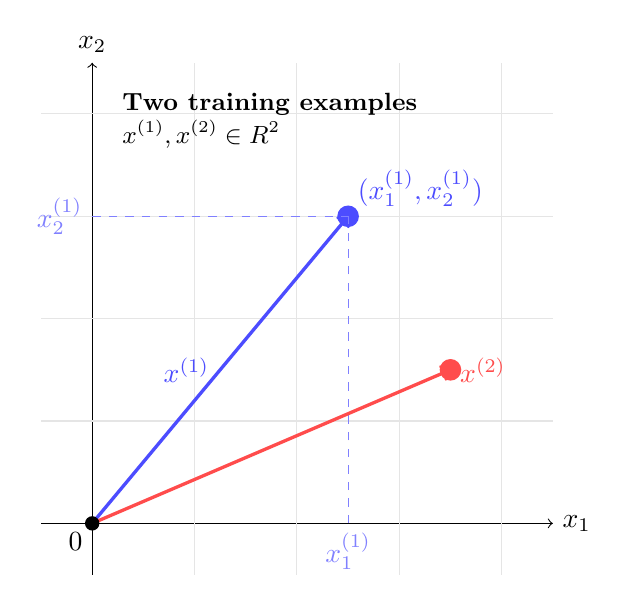
\begin{tikzpicture}[scale=1.3]
        % Coordinate axes
        \draw[->] (-0.5,0) -- (4.5,0) node[right] {$x_1$};
        \draw[->] (0,-0.5) -- (0,4.5) node[above] {$x_2$};

        % Grid (faint)
        \foreach \x in {1,2,3,4} {
                \draw[gray!20] (\x,-0.5) -- (\x,4.5);
                \draw[gray!20] (-0.5,\x) -- (4.5,\x);
            }

        % Vector x^(1)
        \draw[->, very thick, blue!70] (0,0) -- (2.5,3) node[midway, left] {$\vect{x}^{(1)}$};
        \fill[blue!70] (2.5,3) circle (3pt);
        \node[above right, blue!70] at (2.5,3) {$(x_1^{(1)}, x_2^{(1)})$};

        % Projection lines
        \draw[dashed, blue!50] (2.5,0) node[below] {$x_1^{(1)}$} -- (2.5,3);
        \draw[dashed, blue!50] (0,3) node[left] {$x_2^{(1)}$} -- (2.5,3);

        % Vector x^(2)
        \draw[->, very thick, red!70] (0,0) -- (3.5,1.5);
        \fill[red!70] (3.5,1.5) circle (3pt);
        \node[right, red!70] at (3.5,1.5) {$\vect{x}^{(2)}$};

        % Origin
        \fill[black] (0,0) circle (2pt) node[below left] {$\vect{0}$};

        % Annotations
        \node[anchor=north west, align=left] at (0.2,4.3) {
            \small\textbf{Two training examples}\\
            \small$\vect{x}^{(1)}, \vect{x}^{(2)} \in \mathbb{R}^2$
        };
    \end{tikzpicture}

    \textbf{Figure 1:} Geometric representation of vectors as points in $\mathbb{R}^2$. Each vector $\vect{x}^{(i)}$ represents a training example, with components $x_1^{(i)}, x_2^{(i)}$ denoting feature values.
\end{center}

\subsection{Vector Operations: Constructing Structure Through Action}

\begin{necessitybox}
    \textbf{DNR Principle: Necessity}

    New mathematical structures arise from \textit{intellectual need}. We don't
    define operations arbitrarily; we introduce them because they solve problems we
    encounter.

    \textbf{The need for vector addition:} How do we combine two feature vectors? How do we update parameters in gradient descent?

    \textbf{The need for scalar multiplication:} How do we scale a step in optimization? How do we interpolate between examples?

    These questions drive the construction of vector space operations.
\end{necessitybox}

\begin{definition}[Vector Addition]\label{def:vector-addition}
    Let $\vect{u}, \vect{v} \in \mathbb{R}^n$ where:
    \[
        \vect{u} = \begin{bmatrix} u_1 \\ u_2 \\ \vdots \\ u_n \end{bmatrix}, \quad
        \vect{v} = \begin{bmatrix} v_1 \\ v_2 \\ \vdots \\ v_n \end{bmatrix}
    \]

    The \textbf{sum} $\vect{u} + \vect{v} \in \mathbb{R}^n$ is defined
    component-wise:
    \[
        \vect{u} + \vect{v} := \begin{bmatrix} u_1 + v_1 \\ u_2 + v_2 \\ \vdots \\ u_n + v_n \end{bmatrix}
    \]

    \textbf{Closure:} For all $\vect{u}, \vect{v} \in \mathbb{R}^n$, $\vect{u} + \vect{v} \in \mathbb{R}^n$.

    \textbf{Constructive nature:} Given $\vect{u}$ and $\vect{v}$, we construct $\vect{u} + \vect{v}$ by performing $n$ scalar additions.
\end{definition}

\begin{definition}[Scalar Multiplication]\label{def:scalar-mult}
    Let $\vect{v} \in \mathbb{R}^n$ and $\alpha \in \mathbb{R}$. The \textbf{scalar product} $\alpha\vect{v} \in \mathbb{R}^n$ is:
    \[
        \alpha\vect{v} := \begin{bmatrix} \alpha v_1 \\ \alpha v_2 \\ \vdots \\ \alpha v_n \end{bmatrix}
    \]

    \textbf{Closure:} For all $\alpha \in \mathbb{R}$ and $\vect{v} \in \mathbb{R}^n$, $\alpha\vect{v} \in \mathbb{R}^n$.
\end{definition}

\begin{theorem}[Vector Space Axioms for $\mathbb{R}^n$]
    The set $\mathbb{R}^n$ with operations $+$ and scalar multiplication forms a vector space, satisfying:

    \textbf{Addition axioms:}
    \begin{enumerate}
        \item \textbf{Associativity:} $(\vect{u} + \vect{v}) + \vect{w} = \vect{u} + (\vect{v} + \vect{w})$
        \item \textbf{Commutativity:} $\vect{u} + \vect{v} = \vect{v} + \vect{u}$
        \item \textbf{Identity:} $\exists \vect{0} \in \mathbb{R}^n: \vect{v} + \vect{0} = \vect{v}$ for all $\vect{v}$
        \item \textbf{Inverse:} $\forall \vect{v} \in \mathbb{R}^n, \exists (-\vect{v}): \vect{v} + (-\vect{v}) = \vect{0}$
    \end{enumerate}

    \textbf{Scalar multiplication axioms:}
    \begin{enumerate}[resume]
        \item \textbf{Associativity:} $\alpha(\beta\vect{v}) = (\alpha\beta)\vect{v}$
        \item \textbf{Identity:} $1\vect{v} = \vect{v}$
        \item \textbf{Distributivity over vector addition:} $\alpha(\vect{u} + \vect{v}) = \alpha\vect{u} + \alpha\vect{v}$
        \item \textbf{Distributivity over scalar addition:} $(\alpha + \beta)\vect{v} = \alpha\vect{v} + \beta\vect{v}$
    \end{enumerate}
\end{theorem}

\begin{proof}[Proof sketch (constructive)]
    Each axiom is verified by component-wise calculation. For example, commutativity:
    \begin{align*}
        [\vect{u} + \vect{v}]_j & = u_j + v_j \quad \text{(definition of vector addition)}  \\
                                & = v_j + u_j \quad \text{(commutativity of real addition)} \\
                                & = [\vect{v} + \vect{u}]_j
    \end{align*}
    Since this holds for all $j \in \{1, \ldots, n\}$, $\vect{u} + \vect{v} = \vect{v} + \vect{u}$.
\end{proof}

\begin{mlbox}
    \textbf{Machine Learning Application: Gradient Descent Update}

    The fundamental optimization algorithm in ML is gradient descent:
    \[
        \vect{\theta}^{(t+1)} = \vect{\theta}^{(t)} - \alpha \nabla_{\vect{\theta}} J(\vect{\theta}^{(t)})
    \]

    \textbf{Notation breakdown:}
    \begin{itemize}
        \item $\vect{\theta}^{(t)} \in \mathbb{R}^d$: parameter vector at iteration $t$ (superscript = semantic: which iterate)
        \item $\theta_j^{(t)}$: the $j$-th parameter at iteration $t$ (subscript = structural: which component)
        \item $\alpha \in \mathbb{R}_{++}$: learning rate (scalar)
        \item $\nabla_{\vect{\theta}} J(\vect{\theta}^{(t)}) \in \mathbb{R}^d$: gradient vector with components:
              \[
                  [\nabla_{\vect{\theta}} J]_j = \frac{\partial J}{\partial \theta_j}\bigg|_{\vect{\theta} = \vect{\theta}^{(t)}}
              \]
    \end{itemize}

    \textbf{This is vector addition and scalar multiplication:}
    \[
        \vect{\theta}^{(t+1)} = \vect{\theta}^{(t)} + (-\alpha) \nabla_{\vect{\theta}} J(\vect{\theta}^{(t)})
    \]

    The construction is explicit: given $\vect{\theta}^{(0)}$ (initialization), we
    iteratively construct $\vect{\theta}^{(1)}, \vect{\theta}^{(2)}, \ldots$ until
    convergence.
\end{mlbox}

\subsection{The Inner Product: Measuring Similarity and Computing Predictions}

\begin{definition}[Inner Product (Dot Product)]\label{def:inner-product}
    Let $\vect{u}, \vect{v} \in \mathbb{R}^n$. The \textbf{inner product} (or \textbf{dot product}) is the map:
    \[
        \langle \cdot, \cdot \rangle: \mathbb{R}^n \times \mathbb{R}^n \to \mathbb{R}
    \]
    defined by:
    \[
        \langle \vect{u}, \vect{v} \rangle := \sum_{j=1}^{n} u_j v_j = u_1 v_1 + u_2 v_2 + \cdots + u_n v_n
    \]

    \textbf{Alternative notation:}
    \[
        \vect{u} \cdot \vect{v} = \vect{u}^T \vect{v} = \langle \vect{u}, \vect{v} \rangle
    \]

    \textbf{Construction:} Perform $n$ scalar multiplications and $n-1$ scalar additions.
\end{definition}

\begin{theorem}[Properties of the Inner Product]
    The inner product $\langle \cdot, \cdot \rangle: \mathbb{R}^n \times \mathbb{R}^n \to \mathbb{R}$ satisfies:

    \begin{enumerate}
        \item \textbf{Symmetry (Commutativity):}
              \[
                  \langle \vect{u}, \vect{v} \rangle = \langle \vect{v}, \vect{u} \rangle
              \]

        \item \textbf{Linearity in first argument:}
              \[
                  \langle \alpha\vect{u}_1 + \beta\vect{u}_2, \vect{v} \rangle = \alpha\langle \vect{u}_1, \vect{v} \rangle + \beta\langle \vect{u}_2, \vect{v} \rangle
              \]

        \item \textbf{Positive definiteness:}
              \[
                  \langle \vect{v}, \vect{v} \rangle \geq 0, \quad \text{with equality iff } \vect{v} = \vect{0}
              \]
    \end{enumerate}
\end{theorem}

\begin{definition}[Norm Induced by Inner Product]
    The \textbf{Euclidean norm} (or $L^2$ norm) of $\vect{v} \in \mathbb{R}^n$ is:
    \[
        \|\vect{v}\| := \sqrt{\langle \vect{v}, \vect{v} \rangle} = \sqrt{\sum_{j=1}^{n} v_j^2}
    \]

    \textbf{Properties:}
    \begin{enumerate}
        \item $\|\vect{v}\| \geq 0$, with equality iff $\vect{v} = \vect{0}$
        \item $\|\alpha\vect{v}\| = |\alpha|\|\vect{v}\|$
        \item $\|\vect{u} + \vect{v}\| \leq \|\vect{u}\| + \|\vect{v}\|$ (triangle inequality)
    \end{enumerate}
\end{definition}

\begin{theorem}[Cauchy-Schwarz Inequality]
    For all $\vect{u}, \vect{v} \in \mathbb{R}^n$:
    \[
        |\langle \vect{u}, \vect{v} \rangle| \leq \|\vect{u}\| \|\vect{v}\|
    \]
    with equality iff $\vect{u}$ and $\vect{v}$ are linearly dependent.
\end{theorem}

\begin{intuitionbox}
    \textbf{Geometric Interpretation of Inner Product}

    The inner product relates to the angle $\theta \in [0, \pi]$ between vectors:
    \[
        \langle \vect{u}, \vect{v} \rangle = \|\vect{u}\| \|\vect{v}\| \cos\theta
    \]

    \textbf{Cases:}
    \begin{itemize}
    \item $\langle \vect{u}, \vect{v} \rangle > 0$: acute angle ($\theta < \pi/2$), vectors \emph{point similarly}
    \item $\langle \vect{u}, \vect{v} \rangle = 0$: orthogonal ($\theta = \pi/2$), vectors \emph{independent}
    \item $\langle \vect{u}, \vect{v} \rangle < 0$: obtuse angle ($\theta > \pi/2$), vectors \emph{oppose}
    \end{itemize}

    \textbf{ML interpretation:} The inner product measures \textit{similarity} or \textit{alignment}. In recommendation systems, $\langle \vect{u}_{\text{user}}, \vect{v}_{\text{item}} \rangle$ scores how well item $v$ matches user $u$'s preferences.
\end{intuitionbox}

\begin{mlbox}
    \textbf{Linear Regression as Inner Product}

    Prediction for example $i$:
    \[
        \hat{y}^{(i)} = \vect{\theta}^T \vect{x}^{(i)} = \sum_{j=1}^{n} \theta_j x_j^{(i)}
    \]

    \textbf{With bias term:} Augment $\vect{x}^{(i)} \mapsto \tilde{\vect{x}}^{(i)} = [1, x_1^{(i)}, \ldots, x_n^{(i)}]^T \in \mathbb{R}^{n+1}$, $\vect{\theta} \mapsto \tilde{\vect{\theta}} = [\theta_0, \theta_1, \ldots, \theta_n]^T \in \mathbb{R}^{n+1}$:
    \[
        \hat{y}^{(i)} = \tilde{\vect{\theta}}^T \tilde{\vect{x}}^{(i)} = \theta_0 + \sum_{j=1}^{n} \theta_j x_j^{(i)}
    \]

    \textbf{Loss function (Mean Squared Error):}
    \[
        J(\vect{\theta}) = \frac{1}{2m} \sum_{i=1}^{m} \left(\vect{\theta}^T \vect{x}^{(i)} - y^{(i)}\right)^2
    \]

    \textbf{Gradient (using chain rule and linearity):}
    \[
        \frac{\partial J}{\partial \theta_j} = \frac{1}{m} \sum_{i=1}^{m} \left(\vect{\theta}^T \vect{x}^{(i)} - y^{(i)}\right) x_j^{(i)}
    \]

    In vector form:
    \[
        \nabla_{\vect{\theta}} J = \frac{1}{m} \sum_{i=1}^{m} \left(\vect{\theta}^T \vect{x}^{(i)} - y^{(i)}\right) \vect{x}^{(i)}
    \]
\end{mlbox}

\section{Matrices: Encapsulating Linear Transformations}

\subsection{From Vectors to Matrices: The Next Abstraction}

\begin{necessitybox}
    \textbf{Why Do We Need Matrices?}

    Vectors encapsulate data. But machine learning requires \textit{transforming}
    data:
    \begin{itemize}
        \item Rotating feature space
        \item Projecting to lower dimensions (PCA)
        \item Mapping inputs to outputs in neural networks
    \end{itemize}

    \textbf{Question:} How do we represent a linear function $T: \mathbb{R}^n \to \mathbb{R}^m$?

    \textbf{Answer:} Matrices.
\end{necessitybox}

\begin{definition}[Matrix - Constructive Definition]
    \label{def:matrix}
    Let $m, n \in \mathbb{N}$, $m, n \geq 1$. A \textbf{matrix} of size $m \times n$ over $\mathbb{R}$ is a rectangular array:
    \[
        \matr{A} = \begin{bmatrix}
            a_{11} & a_{12} & \cdots & a_{1n} \\
            a_{21} & a_{22} & \cdots & a_{2n} \\
            \vdots & \vdots & \ddots & \vdots \\
            a_{m1} & a_{m2} & \cdots & a_{mn}
        \end{bmatrix} \in \mathbb{R}^{m \times n}
    \]
    where $a_{ij} \in \mathbb{R}$ for $i \in \{1, \ldots, m\}$, $j \in \{1, \ldots,
        n\}$.

    \textbf{Notation conventions:}
    \begin{itemize}
        \item $\matr{A}$ (bold uppercase): the matrix
        \item $a_{ij}$ (lowercase with double subscript): entry in row $i$, column $j$
        \item $\matr{A}_{i,:}$ or $\vect{a}_i^T$: row $i$ (row vector)
        \item $\matr{A}_{:,j}$ or $\vect{a}^{(j)}$: column $j$ (column vector)
    \end{itemize}

    \textbf{Special matrices:}
    \begin{itemize}
        \item \textbf{Square matrix:} $m = n$
        \item \textbf{Zero matrix:} $\matr{0}$: all entries 0
        \item \textbf{Identity matrix:} $\matr{I}_n \in \mathbb{R}^{n \times n}$: $(\matr{I}_n)_{ij} = \delta_{ij}$ (Kronecker delta)
    \end{itemize}
\end{definition}

\begin{notationbox}
    \textbf{Andrew Ng Notation for Neural Network Matrices}

    In a neural network with $L$ layers:

    \textbf{Weight matrix at layer $\ell$:}
    \[
        \matr{W}^{[\ell]} \in \mathbb{R}^{n^{[\ell]} \times n^{[\ell-1]}}
    \]
    \begin{itemize}
        \item $n^{[\ell]}$: number of units in layer $\ell$ (superscript = semantic: which layer)
        \item $W_{jk}^{[\ell]}$: weight from unit $k$ in layer $\ell-1$ to unit $j$ in layer $\ell$
        \item Subscripts $j, k$ denote position in the matrix
    \end{itemize}

    \textbf{Bias vector at layer $\ell$:}
    \[
        \vect{b}^{[\ell]} \in \mathbb{R}^{n^{[\ell]}}, \quad b_j^{[\ell]} = \text{bias for unit } j \text{ in layer } \ell
    \]

    \textbf{Pre-activation:}
    \[
        \vect{z}^{[\ell]} = \matr{W}^{[\ell]} \vect{a}^{[\ell-1]} + \vect{b}^{[\ell]} \in \mathbb{R}^{n^{[\ell]}}
    \]

    \textbf{Activation:}
    \[
        \vect{a}^{[\ell]} = g^{[\ell]}(\vect{z}^{[\ell]}) \in \mathbb{R}^{n^{[\ell]}}
    \]
    where $g^{[\ell]}$ is the activation function (applied element-wise).

    \textbf{Key principle:} Superscripts distinguish \textit{which object} (layer, example); subscripts specify \textit{where within} that object.
\end{notationbox}

\subsection{Matrix Operations}

\begin{definition}[Matrix Addition]
    Let $\matr{A}, \matr{B} \in \mathbb{R}^{m \times n}$. The sum $\matr{A} + \matr{B} \in \mathbb{R}^{m \times n}$ is:
    \[
        (\matr{A} + \matr{B})_{ij} := a_{ij} + b_{ij}, \quad \forall i \in \{1, \ldots, m\}, j \in \{1, \ldots, n\}
    \]

    \textbf{Requirement:} Matrices must have identical dimensions.
\end{definition}

\begin{definition}[Scalar-Matrix Multiplication]
    Let $\alpha \in \mathbb{R}$, $\matr{A} \in \mathbb{R}^{m \times n}$. Then $\alpha\matr{A} \in \mathbb{R}^{m \times n}$ is:
    \[
        (\alpha\matr{A})_{ij} := \alpha a_{ij}
    \]
\end{definition}

\begin{definition}[Matrix-Vector Multiplication]
    \label{def:matrix-vector}
    Let $\matr{A} \in \mathbb{R}^{m \times n}$, $\vect{x} \in \mathbb{R}^n$. The product $\matr{A}\vect{x} \in \mathbb{R}^m$ is defined by:
    \[
        (\matr{A}\vect{x})_i := \sum_{j=1}^{n} a_{ij} x_j = \matr{A}_{i,:} \cdot \vect{x}
    \]

    \textbf{Interpretation 1 (row perspective):} The $i$-th component of $\matr{A}\vect{x}$ is the inner product of row $i$ of $\matr{A}$ with $\vect{x}$.

    \textbf{Interpretation 2 (column perspective):}
    \[
        \matr{A}\vect{x} = \sum_{j=1}^{n} x_j \matr{A}_{:,j} = x_1\vect{a}^{(1)} + x_2\vect{a}^{(2)} + \cdots + x_n\vect{a}^{(n)}
    \]
    where $\vect{a}^{(j)}$ is column $j$ of $\matr{A}$.

    $\matr{A}\vect{x}$ is a \textit{linear combination} of the columns of $\matr{A}$, with coefficients from $\vect{x}$.
\end{definition}

\begin{intuitionbox}
    \textbf{Three Ways to Think About $\matr{A}\vect{x}$}

    \textbf{1. Algebraic:} Sum of products (Definition \ref{def:matrix-vector})

    \textbf{2. Geometric:} $\matr{A}$ transforms vector $\vect{x}$ to $\matr{A}\vect{x}$ (rotation, scaling, projection)

    \textbf{3. ML:} Forward propagation in a linear layer:
    \[
        \vect{z} = \matr{W}\vect{x} + \vect{b}
    \]
    maps input $\vect{x}$ to pre-activation $\vect{z}$.
\end{intuitionbox}

\begin{definition}[Matrix-Matrix Multiplication]
    \label{def:matrix-mult}
    Let $\matr{A} \in \mathbb{R}^{m \times p}$, $\matr{B} \in \mathbb{R}^{p \times n}$. The product $\matr{C} = \matr{A}\matr{B} \in \mathbb{R}^{m \times n}$ is:
    \[
        c_{ij} := \sum_{k=1}^{p} a_{ik} b_{kj}
    \]

    \textbf{Requirement:} Number of columns of $\matr{A}$ equals number of rows of $\matr{B}$.

    \textbf{Interpretation 1 (entry-wise):}
    \[
        c_{ij} = \matr{A}_{i,:} \cdot \matr{B}_{:,j}
    \]
    (inner product of row $i$ of $\matr{A}$ with column $j$ of $\matr{B}$)

    \textbf{Interpretation 2 (column perspective):}
    Column $j$ of $\matr{C}$:
    \[
        \matr{C}_{:,j} = \matr{A} \matr{B}_{:,j}
    \]
    (apply transformation $\matr{A}$ to column $j$ of $\matr{B}$)

    \textbf{Interpretation 3 (row perspective):}
    Row $i$ of $\matr{C}$:
    \[
        \matr{C}_{i,:} = \matr{A}_{i,:} \matr{B}
    \]
\end{definition}

\begin{theorem}[Properties of Matrix Multiplication]
    \label{thm:matrix-mult-props}
    Let $\matr{A}, \matr{B}, \matr{C}$ be matrices of compatible dimensions, $\alpha \in \mathbb{R}$.

    \begin{enumerate}
        \item \textbf{Associativity:} $(\matr{A}\matr{B})\matr{C} = \matr{A}(\matr{B}\matr{C})$
        \item \textbf{Distributivity:} $\matr{A}(\matr{B} + \matr{C}) = \matr{A}\matr{B} + \matr{A}\matr{C}$
        \item \textbf{Scalar compatibility:} $\alpha(\matr{A}\matr{B}) = (\alpha\matr{A})\matr{B} = \matr{A}(\alpha\matr{B})$
        \item \textbf{Identity:} $\matr{I}_m \matr{A} = \matr{A} = \matr{A}\matr{I}_n$ (for $\matr{A} \in \mathbb{R}^{m \times n}$)
    \end{enumerate}

    \textbf{Non-commutativity:} In general, $\matr{A}\matr{B} \neq \matr{B}\matr{A}$.
\end{theorem}

\begin{dualitybox}
    \textbf{DNR Principle: Duality of Concept and Procedure}

    Understanding matrix multiplication requires interplay between:
    \begin{itemize}
        \item \textbf{Conceptual understanding:} Matrix multiplication composes linear transformations
        \item \textbf{Procedural fluency:} Computing $\matr{C} = \matr{A}\matr{B}$ via $c_{ij} = \sum_k a_{ik}b_{kj}$
    \end{itemize}

    Neither alone suffices. The concept explains \textit{why} the procedure works;
    the procedure makes the concept \textit{concrete} and \textit{computable}.

    \textbf{Pedagogical implication:} Introduce both simultaneously, repeatedly connecting abstract meaning to computational steps.
\end{dualitybox}

\subsection{Linear Transformations and Matrix Representations}

\begin{definition}[Linear Transformation]
    \label{def:linear-transformation}
    A function $T: \mathbb{R}^n \to \mathbb{R}^m$ is a \textbf{linear transformation} (or \textbf{linear map}) if for all $\vect{u}, \vect{v} \in \mathbb{R}^n$ and $\alpha, \beta \in \mathbb{R}$:
    \[
        T(\alpha\vect{u} + \beta\vect{v}) = \alpha T(\vect{u}) + \beta T(\vect{v})
    \]

    \textbf{Equivalent conditions:}
    \begin{enumerate}
        \item $T(\vect{u} + \vect{v}) = T(\vect{u}) + T(\vect{v})$ (additivity)
        \item $T(\alpha\vect{v}) = \alpha T(\vect{v})$ (homogeneity)
    \end{enumerate}
\end{definition}

\begin{theorem}[Matrix Representation Theorem]
    \label{thm:matrix-representation}
    Every linear transformation $T: \mathbb{R}^n \to \mathbb{R}^m$ can be represented by a unique matrix $\matr{A} \in \mathbb{R}^{m \times n}$ such that:
    \[
        T(\vect{x}) = \matr{A}\vect{x}, \quad \forall \vect{x} \in \mathbb{R}^n
    \]

    \textbf{Construction of $\matr{A}$:}
    Let $\{\vect{e}_1, \ldots, \vect{e}_n\}$ be the standard basis of $\mathbb{R}^n$ where $\vect{e}_j$ has 1 in position $j$, 0 elsewhere. Then:
    \[
        \text{Column } j \text{ of } \matr{A} = T(\vect{e}_j)
    \]

    \textbf{Verification:}
    For any $\vect{x} = \sum_{j=1}^{n} x_j \vect{e}_j$:
    \[
        T(\vect{x}) = T\left(\sum_{j=1}^{n} x_j \vect{e}_j\right) = \sum_{j=1}^{n} x_j T(\vect{e}_j) = \sum_{j=1}^{n} x_j \matr{A}_{:,j} = \matr{A}\vect{x}
    \]
\end{theorem}

\begin{philobox}
    \textbf{Constructivist Insight: Matrices as Constructed Representations}

    A linear transformation $T$ is an abstract concept—a rule for mapping vectors.
    The matrix $\matr{A}$ is a \textit{constructed representation} of $T$ with
    respect to chosen bases.

    Key points:
    \begin{enumerate}
        \item $T$ exists as a mental construction (the mapping rule)
        \item $\matr{A}$ is a concrete encoding of $T$ (array of numbers)
        \item The encoding depends on basis choice (coordinate systems)
        \item In ML, we often \textit{construct} $T$ by specifying $\matr{A}$ directly (e.g.,
              weight matrices in neural nets)
    \end{enumerate}

    This aligns with constructivism: mathematical objects are built, not
    discovered.
\end{philobox}

\begin{example}[Neural Network Layer as Linear Transformation]
    A single dense layer with $n$ inputs, $m$ outputs (no activation):
    \[
        T: \mathbb{R}^n \to \mathbb{R}^m, \quad T(\vect{x}) = \matr{W}\vect{x} + \vect{b}
    \]

    \textbf{Wait—this is affine, not linear!}

    Correct. But we can make it linear by \textit{homogeneous coordinates}:

    \textbf{Augmentation:}
    \[
        \tilde{\vect{x}} = \begin{bmatrix} \vect{x} \\ 1 \end{bmatrix} \in \mathbb{R}^{n+1}, \quad
        \tilde{\matr{W}} = \begin{bmatrix} \matr{W} & \vect{b} \end{bmatrix} \in \mathbb{R}^{m \times (n+1)}
    \]

    Then:
    \[
        T(\vect{x}) = \tilde{\matr{W}} \tilde{\vect{x}} = \begin{bmatrix} \matr{W} & \vect{b} \end{bmatrix} \begin{bmatrix} \vect{x} \\ 1 \end{bmatrix} = \matr{W}\vect{x} + \vect{b}
    \]

    Now $T$ is represented by a linear map in higher dimension.
\end{example}

\section{Basis, Span, and Linear Independence}

\subsection{Constructing Coordinate Systems}

\begin{definition}[Linear Combination]
    \label{def:linear-combination}
    Let $\vect{v}_1, \ldots, \vect{v}_k \in \mathbb{R}^n$ and $c_1, \ldots, c_k \in \mathbb{R}$. A \textbf{linear combination} of $\{\vect{v}_1, \ldots, \vect{v}_k\}$ is:
    \[
        \vect{v} = c_1\vect{v}_1 + c_2\vect{v}_2 + \cdots + c_k\vect{v}_k = \sum_{j=1}^{k} c_j\vect{v}_j
    \]

    The coefficients $c_1, \ldots, c_k$ are called the \textbf{weights}.
\end{definition}

\begin{intuitionbox}
    \textbf{Linear Combination as Construction}

    A linear combination is an explicit construction: given vectors $\vect{v}_1,
        \ldots, \vect{v}_k$ and scalars $c_1, \ldots, c_k$, we perform:
    \begin{enumerate}
        \item Scale: compute $c_j\vect{v}_j$ for each $j$
        \item Sum: compute $\sum_{j=1}^{k} c_j\vect{v}_j$
    \end{enumerate}

    This is finite, algorithmic, constructive—embodying the constructivist ethos.
\end{intuitionbox}

\begin{definition}[Span]
    \label{def:span}
    The \textbf{span} of vectors $\{\vect{v}_1, \ldots, \vect{v}_k\} \subset \mathbb{R}^n$ is:
    \[
        \text{span}(\vect{v}_1, \ldots, \vect{v}_k) := \left\{ \sum_{j=1}^{k} c_j\vect{v}_j : c_1, \ldots, c_k \in \mathbb{R} \right\}
    \]

    \textbf{Interpretation:} The set of all vectors that can be constructed as linear combinations of $\vect{v}_1, \ldots, \vect{v}_k$.

    \textbf{Fact:} $\text{span}(\vect{v}_1, \ldots, \vect{v}_k)$ is a subspace of $\mathbb{R}^n$.
\end{definition}

\begin{definition}[Linear Independence]
    \label{def:linear-independence}
    Vectors $\vect{v}_1, \ldots, \vect{v}_k \in \mathbb{R}^n$ are \textbf{linearly independent} if the only solution to:
    \[
        c_1\vect{v}_1 + c_2\vect{v}_2 + \cdots + c_k\vect{v}_k = \vect{0}
    \]
    is $c_1 = c_2 = \cdots = c_k = 0$.

    \textbf{Contrapositive (Linear Dependence):} If there exist $c_1, \ldots, c_k$ not all zero such that $\sum_{j=1}^{k} c_j\vect{v}_j = \vect{0}$, the vectors are \textbf{linearly dependent}.
\end{definition}

\begin{intuitionbox}
    \textbf{Geometric Intuition}

    	extbf{Linear independence:} No vector is redundant; each adds a \emph{new direction}.

    \textbf{Linear dependence:} At least one vector can be expressed in terms of others (redundancy).

    \textbf{Example in $\mathbb{R}^2$:}
    \begin{itemize}
        \item $\vect{v}_1 = \begin{bmatrix} 1 \\ 0 \end{bmatrix}, \vect{v}_2 = \begin{bmatrix} 0 \\ 1 \end{bmatrix}$: independent (span all of $\mathbb{R}^2$)
        \item $\vect{v}_1 = \begin{bmatrix} 1 \\ 2 \end{bmatrix}, \vect{v}_2 = \begin{bmatrix} 2 \\ 4 \end{bmatrix}$: dependent ($\vect{v}_2 = 2\vect{v}_1$)
    \end{itemize}
\end{intuitionbox}

\begin{definition}[Basis]
    \label{def:basis}
    A set $\{\vect{b}_1, \ldots, \vect{b}_n\} \subset \mathbb{R}^n$ is a \textbf{basis} for $\mathbb{R}^n$ if:
    \begin{enumerate}
        \item \textbf{Span condition:} $\text{span}(\vect{b}_1, \ldots, \vect{b}_n) = \mathbb{R}^n$
        \item \textbf{Independence condition:} $\vect{b}_1, \ldots, \vect{b}_n$ are linearly independent
    \end{enumerate}

    \textbf{Equivalent characterization:} Every $\vect{v} \in \mathbb{R}^n$ can be uniquely written as:
    \[
        \vect{v} = c_1\vect{b}_1 + \cdots + c_n\vect{b}_n
    \]

    The coefficients $(c_1, \ldots, c_n)$ are the \textbf{coordinates} of
    $\vect{v}$ with respect to basis $\{\vect{b}_1, \ldots, \vect{b}_n\}$.
\end{definition}

\begin{theorem}[Dimension]
    All bases of $\mathbb{R}^n$ have exactly $n$ vectors. This common number is the \textbf{dimension} of $\mathbb{R}^n$:
    \[
        \dim(\mathbb{R}^n) = n
    \]
\end{theorem}

\begin{example}[Standard Basis]
    The \textbf{standard basis} of $\mathbb{R}^n$ is:
    \[
        \mathcal{E} = \{\vect{e}_1, \vect{e}_2, \ldots, \vect{e}_n\}
    \]
    where:
    \[
        \vect{e}_j = \begin{bmatrix} 0 \\ \vdots \\ 0 \\ 1 \\ 0 \\ \vdots \\ 0 \end{bmatrix} \leftarrow \text{1 in position } j
    \]

    Any $\vect{x} = [x_1, \ldots, x_n]^T$ is:
    \[
        \vect{x} = \sum_{j=1}^{n} x_j \vect{e}_j
    \]

    The coordinates of $\vect{x}$ in standard basis are simply $(x_1, \ldots,
        x_n)$.
\end{example}

\begin{center}
    \begin{tikzpicture}[scale=1.8]
        % Axes
        \draw[->] (-0.3,0) -- (3.5,0) node[right] {$x_1$};
        \draw[->] (0,-0.3) -- (0,3.5) node[above] {$x_2$};

        % Standard basis vectors
        \draw[->, very thick, red] (0,0) -- (2,0) node[midway, below] {$\vect{e}_1$};
        \draw[->, very thick, blue] (0,0) -- (0,2) node[midway, left] {$\vect{e}_2$};

        % A general vector
        \draw[->, very thick, green!60!black] (0,0) -- (2.5,1.5) node[midway, above left] {$\vect{x}$};

        % Projections
        \draw[dashed, gray] (2.5,0) -- (2.5,1.5);
        \draw[dashed, gray] (0,1.5) -- (2.5,1.5);

        % Decomposition
        \draw[->, thick, red!70] (0,0) -- (2.5,0) node[midway, below] {$x_1\vect{e}_1$};
        \draw[->, thick, blue!70] (2.5,0) -- (2.5,1.5) node[midway, right] {$x_2\vect{e}_2$};

        % Labels
        \node at (2.5,-0.3) {$x_1$};
        \node at (-0.3,1.5) {$x_2$};

        \node[anchor=north west] at (0.2,3.3) {
            \small $\vect{x} = x_1\vect{e}_1 + x_2\vect{e}_2$
        };
    \end{tikzpicture}

    \textbf{Figure 2:} Decomposition of vector $\vect{x}$ in standard basis $\{\vect{e}_1, \vect{e}_2\}$ of $\mathbb{R}^2$.
\end{center}

\subsection{Change of Basis and Coordinate Transformations}

\begin{necessitybox}
    \textbf{Why Change Basis?}

    In many ML applications, the standard basis is not optimal:
    \begin{itemize}
        \item \textbf{PCA:} Find basis aligned with directions of maximum variance
        \item \textbf{Fourier transform:} Change from time basis to frequency basis
        \item \textbf{Feature engineering:} Transform to basis where classes are linearly separable
    \end{itemize}

    \textbf{Question:} Given coordinates in one basis, how do we compute coordinates in another basis?
\end{necessitybox}

\begin{theorem}[Change of Basis Formula]
    \label{thm:change-of-basis}
    Let $\mathcal{B} = \{\vect{b}_1, \ldots, \vect{b}_n\}$ and $\mathcal{B}' = \{\vect{b}'_1, \ldots, \vect{b}'_n\}$ be two bases of $\mathbb{R}^n$.

    Let $[\vect{v}]_{\mathcal{B}}$ denote coordinates of $\vect{v}$ in basis
    $\mathcal{B}$.

    The \textbf{change-of-basis matrix} from $\mathcal{B}$ to $\mathcal{B}'$ is:
    \[
        \matr{P}_{\mathcal{B} \to \mathcal{B}'} := \begin{bmatrix} [\vect{b}_1]_{\mathcal{B}'} & [\vect{b}_2]_{\mathcal{B}'} & \cdots & [\vect{b}_n]_{\mathcal{B}'} \end{bmatrix}
    \]

    Then for any $\vect{v} \in \mathbb{R}^n$:
    \[
        [\vect{v}]_{\mathcal{B}'} = \matr{P}_{\mathcal{B} \to \mathcal{B}'} [\vect{v}]_{\mathcal{B}}
    \]
\end{theorem}

\begin{proof}[Proof (constructive)]
    Write $\vect{v}$ in basis $\mathcal{B}$:
    \[
        \vect{v} = \sum_{j=1}^{n} c_j \vect{b}_j, \quad c_j = [[\vect{v}]_{\mathcal{B}}]_j
    \]

    Express each $\vect{b}_j$ in basis $\mathcal{B}'$:
    \[
        \vect{b}_j = \sum_{k=1}^{n} p_{kj} \vect{b}'_k, \quad \text{where } p_{kj} = [[\vect{b}_j]_{\mathcal{B}'}]_k
    \]

    Substitute:
    \begin{align*}
        \vect{v} & = \sum_{j=1}^{n} c_j \left(\sum_{k=1}^{n} p_{kj} \vect{b}'_k\right) \\
                 & = \sum_{k=1}^{n} \left(\sum_{j=1}^{n} p_{kj} c_j\right) \vect{b}'_k
    \end{align*}

    Thus:
    \[
        [[\vect{v}]_{\mathcal{B}'}]_k = \sum_{j=1}^{n} p_{kj} c_j = (\matr{P}_{\mathcal{B} \to \mathcal{B}'} [\vect{v}]_{\mathcal{B}})_k
    \]

    Hence: $[\vect{v}]_{\mathcal{B}'} = \matr{P}_{\mathcal{B} \to \mathcal{B}'}
            [\vect{v}]_{\mathcal{B}}$.
\end{proof}

\subsection{Covariance and Contravariance}

\begin{philobox}
    \textbf{Covariant vs. Contravariant Quantities}

    In differential geometry and tensor analysis, quantities transform differently
    under coordinate changes:

    \textbf{Contravariant vectors} (e.g., position, velocity): Transform \textit{inversely} to basis change.

    \textbf{Covariant vectors} (e.g., gradients, dual vectors): Transform \textit{with} basis change.

    \textbf{Why does this matter in ML?}

    When we change coordinates (e.g., via PCA), we must track how different
    quantities transform:
    \begin{itemize}
        \item Data vectors $\vect{x}^{(i)}$: contravariant (transform with $\matr{P}^{-1}$)
        \item Gradients $\nabla_{\vect{x}} f$: covariant (transform with $\matr{P}^T$)
    \end{itemize}

    This ensures invariance of inner products and optimization steps.
\end{philobox}

\begin{definition}[Covariant and Contravariant Transformation]
    Under change of basis with matrix $\matr{P}$:

    \textbf{Contravariant (vector) transformation:}
    \[
        \vect{v}' = \matr{P}^{-1} \vect{v}
    \]

    \textbf{Covariant (dual vector/gradient) transformation:}
    \[
        \vect{\omega}' = \matr{P}^T \vect{\omega}
    \]

    \textbf{Invariance of pairing:}
    \[
        \vect{\omega}^T \vect{v} = (\vect{\omega}')^T \vect{v}' = (\matr{P}^T\vect{\omega})^T (\matr{P}^{-1}\vect{v}) = \vect{\omega}^T \vect{v}
    \]
\end{definition}

\section{Fundamental Concepts: Kernel, Range, and Rank}

\subsection{The Kernel (Null Space)}

\begin{definition}[Kernel/Null Space]
    \label{def:kernel}
    Let $\matr{A} \in \mathbb{R}^{m \times n}$. The \textbf{kernel} (or \textbf{null space}) of $\matr{A}$ is:
    \[
        \ker(\matr{A}) := \{\vect{x} \in \mathbb{R}^n : \matr{A}\vect{x} = \vect{0}\} \subset \mathbb{R}^n
    \]

    	extbf{Interpretation:} Vectors that are \emph{annihilated} by the linear map $\matr{A}$.

    \textbf{Fact:} $\ker(\matr{A})$ is a subspace of $\mathbb{R}^n$.
\end{definition}

\begin{definition}[Nullity]
    The \textbf{nullity} of $\matr{A}$ is:
    \[
        \text{nullity}(\matr{A}) := \dim(\ker(\matr{A}))
    \]
\end{definition}

\begin{intuitionbox}
    \textbf{Geometric Meaning of Kernel}

    $\ker(\matr{A})$ represents the \emph{directions of collapse}: input directions that map to the zero vector.

    \textbf{Example:} Projection onto $xy$-plane in $\mathbb{R}^3$:
    \[
        \matr{P} = \begin{bmatrix} 1 & 0 & 0 \\ 0 & 1 & 0 \\ 0 & 0 & 0 \end{bmatrix}
    \]

    $\ker(\matr{P}) = \text{span}\left(\begin{bmatrix} 0 \\ 0 \\ 1 \end{bmatrix}\right)$ (the $z$-axis is collapsed).
\end{intuitionbox}

\subsection{The Range (Column Space)}

\begin{definition}[Range/Column Space]
    \label{def:range}
    Let $\matr{A} \in \mathbb{R}^{m \times n}$. The \textbf{range} (or \textbf{column space}) of $\matr{A}$ is:
    \[
        \text{range}(\matr{A}) := \{\matr{A}\vect{x} : \vect{x} \in \mathbb{R}^n\} = \text{span}(\vect{a}^{(1)}, \ldots, \vect{a}^{(n)}) \subset \mathbb{R}^m
    \]
    where $\vect{a}^{(j)}$ is column $j$ of $\matr{A}$.

    \textbf{Interpretation:} All possible outputs of $\matr{A}$.

    \textbf{Fact:} $\text{range}(\matr{A})$ is a subspace of $\mathbb{R}^m$.
\end{definition}

\begin{definition}[Rank]
    \label{def:rank}
    The \textbf{rank} of $\matr{A}$ is:
    \[
        \text{rank}(\matr{A}) := \dim(\text{range}(\matr{A}))
    \]

    \textbf{Equivalent characterization:} Maximum number of linearly independent columns of $\matr{A}$ (equals maximum number of linearly independent rows).
\end{definition}

\begin{theorem}[Rank-Nullity Theorem]
    \label{thm:rank-nullity}
    Let $\matr{A} \in \mathbb{R}^{m \times n}$. Then:
    \[
        \text{rank}(\matr{A}) + \text{nullity}(\matr{A}) = n
    \]

    \textbf{Interpretation:} The input space $\mathbb{R}^n$ decomposes as:
    \[
        \mathbb{R}^n = \ker(\matr{A}) \oplus V
    \]
    where $V$ is a complement, and $\dim(V) = \text{rank}(\matr{A})$.
\end{theorem}

\begin{mlbox}
    \textbf{ML Interpretation: Feature Selection and Dimensionality}

    Consider data matrix $\matr{X} \in \mathbb{R}^{m \times n}$ ($m$ examples, $n$
    features).

    $\text{rank}(\matr{X}) = r < n$ implies:
    \begin{itemize}
        \item Only $r$ features are truly independent
        \item Remaining $n - r$ features are redundant (linear combinations of others)
        \item We can reduce to $r$ dimensions without information loss
    \end{itemize}

    This motivates PCA, which finds an orthonormal basis for
    $\text{range}(\matr{X}^T)$, ordered by importance.
\end{mlbox}

\subsection{Row Reduction as Conceptual Tool}

\begin{dualitybox}
    \textbf{DNR Principle: Row Reduction as Reasoning Tool}

    Row reduction (Gaussian elimination) is typically taught as an
    \textit{algorithm} to solve $\matr{A}\vect{x} = \vect{b}$.

    \textbf{Deeper role:} Row reduction is a \textit{conceptual tool} for understanding:
    \begin{itemize}
        \item Rank (number of pivots)
        \item Kernel (free variables give basis)
        \item Linear independence (do rows reduce to zero?)
        \item Invertibility (is reduced form $\matr{I}$?)
    \end{itemize}

    \textbf{Pedagogical strategy:} Teach row reduction not just as computation, but as a \textit{way of reasoning} about linear systems.
\end{dualitybox}

\begin{definition}[Row Echelon Form (REF)]
    Matrix $\matr{U}$ is in \textbf{row echelon form} if:
    \begin{enumerate}
        \item All zero rows are at the bottom
        \item The first nonzero entry (pivot) of each row is to the right of the pivot of the
              row above
        \item All entries below pivots are zero
    \end{enumerate}
\end{definition}

\begin{definition}[Reduced Row Echelon Form (RREF)]
    Matrix $\matr{R}$ is in \textbf{reduced row echelon form} if:
    \begin{enumerate}
        \item $\matr{R}$ is in REF
        \item Each pivot equals 1
        \item All entries above each pivot are zero
    \end{enumerate}

    \textbf{Uniqueness:} Every matrix has a unique RREF.
\end{definition}

\begin{theorem}[Row Reduction Preserves Rank]
    \label{thm:row-reduction-rank}
    Let $\matr{A} \in \mathbb{R}^{m \times n}$, and let $\matr{U}$ be its REF. Then:
    \[
        \text{rank}(\matr{A}) = \text{number of pivots in } \matr{U}
    \]

    \textbf{Reasoning:} Row operations are left-multiplication by invertible matrices:
    \[
        \matr{E}_k \cdots \matr{E}_1 \matr{A} = \matr{U}
    \]
    where each $\matr{E}_i$ is elementary (invertible). Since invertible maps
    preserve rank:
    \[
        \text{rank}(\matr{U}) = \text{rank}(\matr{A})
    \]

    Pivots in $\matr{U}$ directly count linearly independent rows.
\end{theorem}

\begin{example}[Computing Kernel via RREF]
    Given:
    \[
        \matr{A} = \begin{bmatrix} 1 & 2 & 3 \\ 2 & 4 & 6 \\ 1 & 1 & 2 \end{bmatrix}
    \]

    \textbf{Step 1:} Row reduce to RREF:
    \[
        \text{RREF}(\matr{A}) = \begin{bmatrix} 1 & 0 & 1 \\ 0 & 1 & 1 \\ 0 & 0 & 0 \end{bmatrix}
    \]

    \textbf{Step 2:} Identify free variables. Pivots in columns 1, 2; column 3 is free.

    \textbf{Step 3:} Write $\matr{A}\vect{x} = \vect{0}$ in terms of RREF:
    \[
        \begin{bmatrix} 1 & 0 & 1 \\ 0 & 1 & 1 \\ 0 & 0 & 0 \end{bmatrix} \begin{bmatrix} x_1 \\ x_2 \\ x_3 \end{bmatrix} = \begin{bmatrix} 0 \\ 0 \\ 0 \end{bmatrix}
    \]

    Gives: $x_1 + x_3 = 0$, $x_2 + x_3 = 0$. Set $x_3 = t$ (free parameter):
    \[
        \vect{x} = \begin{bmatrix} -t \\ -t \\ t \end{bmatrix} = t \begin{bmatrix} -1 \\ -1 \\ 1 \end{bmatrix}
    \]

    Thus:
    \[
        \ker(\matr{A}) = \text{span}\left(\begin{bmatrix} -1 \\ -1 \\ 1 \end{bmatrix}\right), \quad \text{nullity}(\matr{A}) = 1
    \]

    And: $\text{rank}(\matr{A}) = 2$, confirming $2 + 1 = 3$.
\end{example}

\section{Eigenvalues, Eigenvectors, and Diagonalization}

\subsection{Invariant Directions: The Essence of Eigenvectors}

\begin{necessitybox}
    \textbf{Why Eigenvalues?}

    Many ML algorithms involve repeated application of a transformation:
    \begin{itemize}
        \item Power iteration for PageRank
        \item Markov chains (transition matrices)
        \item Iterative optimization (Hessian analysis)
    \end{itemize}

    \textbf{Question:} What happens to vectors under repeated application of $\matr{A}$?

    \textbf{Key insight:} Some special vectors only get scaled, not rotated—these are eigenvectors.
\end{necessitybox}

\begin{definition}[Eigenvalue and Eigenvector]
    \label{def:eigenvalue}
    Let $\matr{A} \in \mathbb{R}^{n \times n}$. A scalar $\lambda \in \mathbb{R}$ (or $\mathbb{C}$) is an \textbf{eigenvalue} of $\matr{A}$ if there exists a nonzero vector $\vect{v} \in \mathbb{R}^n$ ($\vect{v} \neq \vect{0}$) such that:
    \[
        \matr{A}\vect{v} = \lambda\vect{v}
    \]

    The vector $\vect{v}$ is called an \textbf{eigenvector} corresponding to
    $\lambda$.

    \textbf{Geometric meaning:} $\matr{A}$ acts on $\vect{v}$ by pure scaling (no rotation), with scale factor $\lambda$.
\end{definition}

\begin{center}
\begin{tikzpicture}[scale=2]
% Original vector v
\draw[->, very thick, blue] (0,0) -- (1,0.5) node[midway, above] {$\vect{v}$};
\fill[blue] (1,0.5) circle (1.5pt);

% After transformation Av = lambda v (lambda = 2)
\draw[->, very thick, red] (0,0) -- (2,1) node[midway, below] {$\matr{A}\vect{v}$};
\fill[red] (2,1) circle (1.5pt);

% Axes
\draw[->] (-0.5,0) -- (2.5,0) node[right] {$x$};
\draw[->] (0,-0.5) -- (0,1.5) node[above] {$y$};
\end{tikzpicture}
\end{center}